\documentclass[aspectratio=169]{beamer}
\usetheme{Boadilla}
\usecolortheme{seahorse}
\usepackage[T1]{fontenc}
\usepackage{lmodern}
\usepackage{booktabs}
\usepackage{xcolor}
\usepackage{tikz}
\usepackage{pgfplots}
\pgfplotsset{compat=1.17}
\usetikzlibrary{arrows.meta,positioning,fit,backgrounds}

\setbeamertemplate{navigation symbols}{}
\setbeamertemplate{itemize items}[circle]
\graphicspath{{../writeup-20261012-111337/handwritten/}}

\newcommand{\keybox}[1]{%
  \begin{center}
  \colorbox{black!8}{\parbox{0.92\textwidth}{\centering #1}}
  \end{center}}
\newcommand{\goodbox}[1]{%
  \begin{center}
  \colorbox{green!12}{\parbox{0.92\textwidth}{\centering #1}}
  \end{center}}

\title{Colibri}
\subtitle{GLM-5.2 at int4 on one GPU --- a frontier model that can read the data}
\author{\texttt{libr-local-llm}}
\date{}

\begin{document}

\frame{\titlepage}

%----------------------------------------------------------
\begin{frame}{Which server is Colibri?}

Three servers were put in front of us. Exactly one is Colibri.

\vspace{0.5em}
\begin{center}
\small
\renewcommand{\arraystretch}{1.4}
\begin{tabular}{@{}p{0.40\textwidth}p{0.52\textwidth}@{}}
\toprule
\textbf{Candidate} & \textbf{Why it is not Colibri} \\
\midrule
gpt-oss:120b, IT's VM, HTTPS & wrong model \emph{and} wrong place: not GLM-5.2, not a c3\_short node \\
qwen3-coder:30b, ollama, loopback & wrong model: not GLM-5.2 \\
\textbf{GLM-5.2 int4, one GPU, c3\_short} & \textbf{this is Colibri} \\
\bottomrule
\end{tabular}
\end{center}

\end{frame}

%----------------------------------------------------------
\begin{frame}{How a 400\,GB model fits on a 46\,GB card}

\begin{columns}[T]
\begin{column}{0.52\textwidth}
\small
A token cannot carry the whole model, so Colibri splits it in two:
\begin{itemize}
\item \textbf{$\approx 23$\,GB} of dense and attention tensors plus the KV cache stay \textbf{resident} in the A40's 46\,GB of VRAM. Every token reads all of it.
\item \textbf{$\approx 407$\,GB} of routed experts wait in the node's \textbf{1\,TB of RAM}, fetched into the card only for the tokens that need them.
\end{itemize}
\end{column}
\begin{column}{0.44\textwidth}
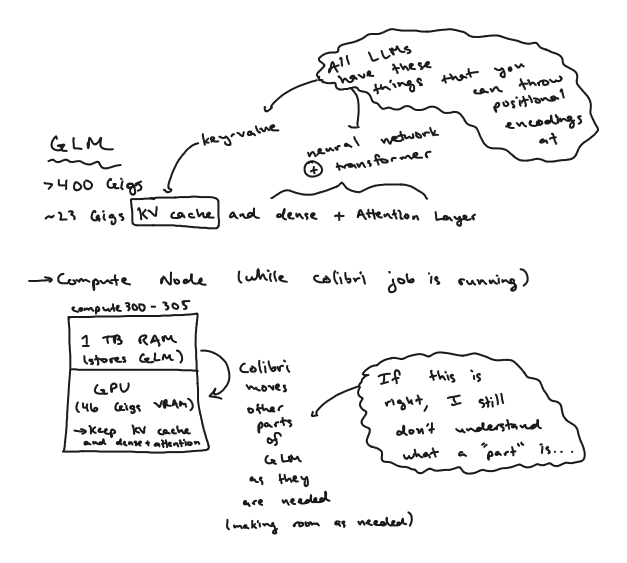
\includegraphics[width=\textwidth,height=0.66\textheight,keepaspectratio]{writeup-20261012-111337-colibri-resident-set.png}
\end{column}
\end{columns}

\end{frame}

%----------------------------------------------------------
\begin{frame}{What a part is}

\begin{columns}[T]
\begin{column}{0.52\textwidth}
\small
\textbf{A part is one routed expert's weights} --- one block in the 407\,GB bank. A token lights only a few of them, so each block can be chosen and moved on its own.

\vspace{0.6em}
The 23\,GB resident set has \textbf{no parts}: every token reads all of it, so nothing inside it ever splits off into a piece that can be selected or moved.
\end{column}
\begin{column}{0.44\textwidth}
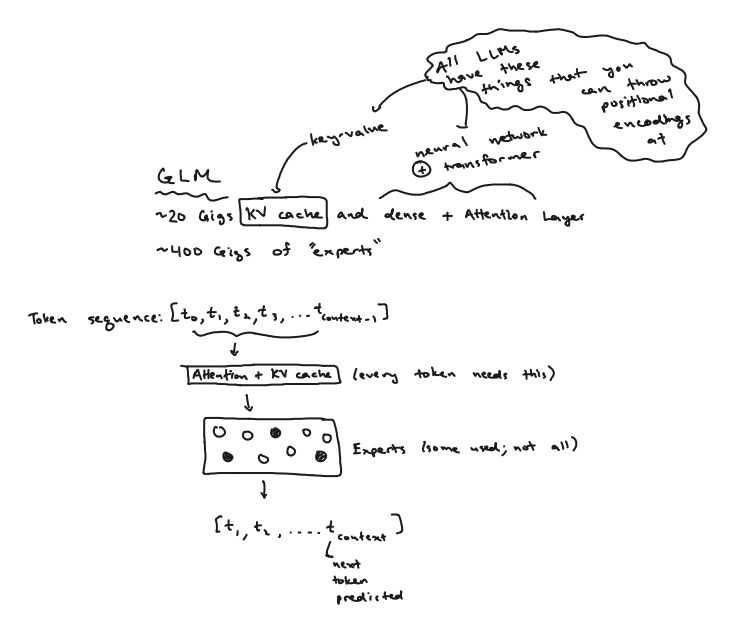
\includegraphics[width=\textwidth,height=0.66\textheight,keepaspectratio]{writeup-20261012-111337-colibri-part.png}
\end{column}
\end{columns}

\end{frame}

%----------------------------------------------------------
\begin{frame}{The fetch}

\begin{columns}[T]
\begin{column}{0.52\textwidth}
\small
One thing travels across the gap: \textbf{a routed expert's weights}, one part.

\vspace{0.6em}
It rests in the node's 1\,TB of RAM and is copied into the A40's VRAM when a token routes to it. The card is far too small to hold every expert, so only the parts a token actually needs cross over --- and room is made for them as they come.
\end{column}
\begin{column}{0.44\textwidth}
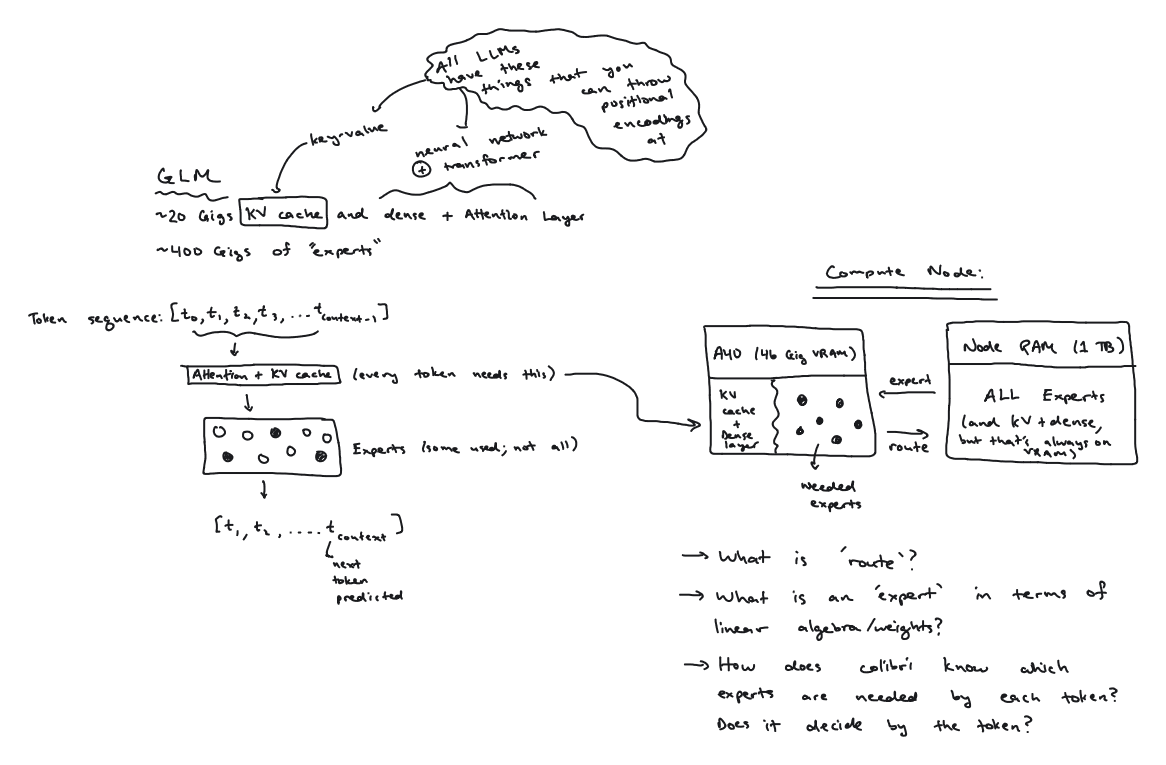
\includegraphics[width=\textwidth,height=0.66\textheight,keepaspectratio]{writeup-20261012-111337-colibri-what-travels.png}
\end{column}
\end{columns}

\end{frame}

%----------------------------------------------------------
\begin{frame}{One token touches 600 expert-weights}

\begin{columns}[T]
\begin{column}{0.56\textwidth}
\small
GLM-5.2 has \textbf{75 MoE blocks}, each holding its own \textbf{256} routed experts, and no two blocks share experts. A token keeps the top $\mathbf{k=8}$ experts in \emph{every} block.

\vspace{0.8em}
\[
75 \times 8 = 600
\]
one token's active expert-weights per forward pass, out of the model's $256\times75=19{,}200$ routed experts.
\end{column}
\begin{column}{0.40\textwidth}
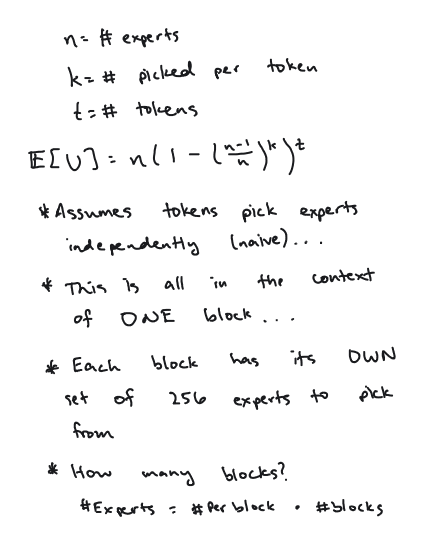
\includegraphics[width=\textwidth,height=0.66\textheight,keepaspectratio]{writeup-20261012-111337-colibri-expert-weights.png}
\end{column}
\end{columns}

\end{frame}

%----------------------------------------------------------
\begin{frame}{Two tokens, one pass: read the union}

\begin{columns}[T]
\begin{column}{0.54\textwidth}
\small
\begin{tabular}{@{}ll@{}}
\toprule
Token A & $\{3,17,42,88,101,150,200,255\}$ \\
Token B & $\{8,17,42,60,99,101,200,255\}$ \\
\bottomrule
\end{tabular}

\vspace{0.7em}
They share $\{17,42,101,200,255\}$ --- five experts --- so the block reads
\[
8+8-5 = 11
\]
distinct experts for the two tokens together: $11/2=5.5$ per token, below the $8$ a single token reads.
\end{column}
\begin{column}{0.42\textwidth}
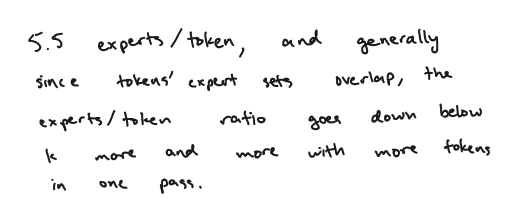
\includegraphics[width=\textwidth,height=0.66\textheight,keepaspectratio]{writeup-20261012-111337-colibri-expert-union.png}
\end{column}
\end{columns}

\end{frame}

%----------------------------------------------------------
\begin{frame}{The formula}

\begin{columns}[T]
\begin{column}{0.52\textwidth}
\small
One block holds $n$ experts; each token keeps $k$ of them, chosen independently; $t$ tokens share one forward pass.

\vspace{0.6em}
By linearity over the $n$ experts, each missed by every token with probability $\bigl(\tfrac{n-k}{n}\bigr)^t$:
\[
E[U] = n\Bigl(1-\bigl(\tfrac{n-k}{n}\bigr)^{t}\Bigr)
\]
The exponent $t$ counts the tokens sharing the pass.
\end{column}
\begin{column}{0.44\textwidth}
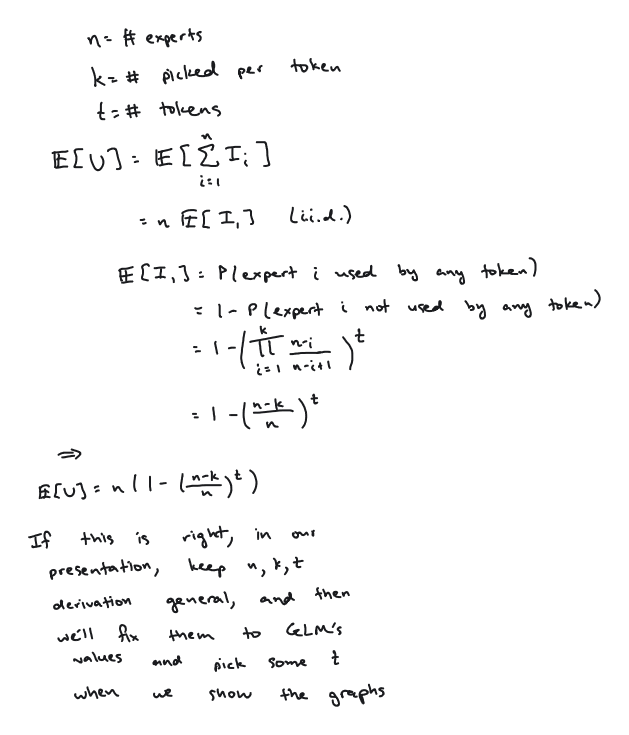
\includegraphics[width=\textwidth,height=0.66\textheight,keepaspectratio]{writeup-20261012-111337-colibri-union-formula.png}
\end{column}
\end{columns}

\end{frame}

%----------------------------------------------------------
\begin{frame}{The verdict: batching barely pays}

\begin{columns}[T]
\begin{column}{0.52\textwidth}
\small
Put in GLM's numbers, $n=256$ and $k=8$:
\[
E[U] = 256\Bigl(1-(31/32)^{t}\Bigr)
\]
At $t=2$ the block reads $E[U]=15.75$ distinct experts --- against a ceiling of $2k=16$.

\vspace{0.6em}
So batching is neither free ($E[U]>8$) nor useless ($E[U]<16$): two tokens share almost none of their experts, and only a sliver ($16-15.75=0.25$) is saved.
\end{column}
\begin{column}{0.46\textwidth}
\begin{tikzpicture}
\begin{axis}[
  width=\textwidth, height=0.62\textheight,
  xlabel={tokens per pass $t$}, ylabel={distinct experts $E[U]$},
  domain=1:64, samples=80, xmin=1, xmax=64, ymin=0, ymax=68,
  grid=both, tick label style={font=\tiny}, label style={font=\small},
  legend style={font=\tiny, at={(0.98,0.02)}, anchor=south east}]
\addplot[very thick, blue!70!black] {256*(1-(31/32)^x)};
\addlegendentry{$E[U]=256\bigl(1-(31/32)^t\bigr)$}
\addplot[dashed, red!70!black, domain=1:64] {16};
\addlegendentry{ceiling $2k=16$}
\addplot[only marks, mark=*, mark size=1.6pt, black] coordinates {(2,15.75)};
\end{axis}
\end{tikzpicture}
\end{column}
\end{columns}

\end{frame}

%----------------------------------------------------------
\begin{frame}{Why it can read the data}

\small
Colibri is allowed to touch therapy recordings because it runs on LIBR hardware and never leaves it. The on-disk transcript is what has to be guarded, so it is written \emph{inside} a directory named \texttt{phi}.

\vspace{0.7em}
The front end writes its transcript under a folder named for the \emph{program}, and the local driver roots that folder inside \texttt{phi}:
\begin{itemize}
\item driven through \texttt{claude}, the transcript lands at \texttt{\$COLI\_SESSION\_ROOT/phi/claude/\ldots}
\item driven through \texttt{opencode}, the same path reads \texttt{\$COLI\_SESSION\_ROOT/phi/opencode/\ldots}
\end{itemize}

\vspace{0.4em}
The fence matches a directory named \texttt{phi} by name, at any depth, so the transcript is refused to every hosted assistant and readable only by the local model.

\end{frame}

%----------------------------------------------------------
\begin{frame}{So what}

\goodbox{\large GLM-5.2 at int4 on \textbf{one GPU}, RAM-backed and local --- a frontier model the lab can point at its own data, because nothing it reads ever leaves the building.}

\vspace{0.9em}
\keybox{Batching barely pays: two tokens read almost their full $2k=16$ experts, $15.75$ against a ceiling of $16$. The lever is the ratio $k/n=8/256$.}

\end{frame}

\end{document}
